92. $f(x)=\cfrac{x^2+x}{x}\cdot\sqrt{x^2-6x+9}=\cfrac{x(x+1)}{x}\cdot\sqrt{(x-3)^2}=\begin{cases}(x+1)|x-3|,\\ x\neq0.\end{cases}=$\\$
\begin{cases}x^2-2x-3,\ x\geqslant3,\\ -x^2+2x+3,\ x\in(-\infty;0)\cup(0;3).\end{cases}$
$$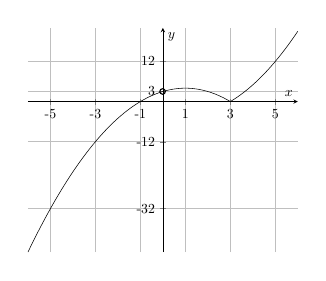
\begin{tikzpicture}[scale=0.5]
\begin{axis}[
    axis lines = middle,
    grid=major,
    legend pos={south west},
    xlabel = {$x$},
    %xlabel style={below right},
    ylabel = {$y$},
    ymin=-45,
    ymax=22,
    xmin=-6,
    xmax=6,
    xtick={-5,-3,-1, 1,3,5},
    xticklabels={-5,-3,-1, 1,3,5},
    ytick={-32,-12,3,12},
    yticklabels={-32,-12,3,12},
                  ]
	\addplot[domain=3:6, samples=100, color=black] {(x*x-2*x-3)};
\addplot[domain=-6:3, samples=100, color=black] {(-x*x+2*x+3)};
        %\addplot[domain=2.01:6, samples=100, color=black] {2/(2-x)};
   % \addplot[domain=-3:3, samples=100, color=black] {-x};
     %\addlegendentry{$\text{Рис. 1}$};
\end{axis}
\draw (3.42,4.08) circle (2pt);
\end{tikzpicture}$$
